\section{Tierra Pirata}

\subsection{Memory Management Functions}
Para facilitar el manejo del armado de estructuras para la paginación, se crearon las siguientes funciones en C. Antes de explicar que hace cada función, un comentario. Cada directorio de paginas tiene 1024 entradas de descriptores de 4 bytes. Lo mismo sucede con los directorios de paginas, que también tienen 1024 entradas con descriptores de 4 bytes. El procesador, al buscar estas estructuras en memoria RAM, requiere que las mismas estén alineadas a 4kb, dado que es el tamaño de pagina que carga en memoria cache.

\begin{enumerate}
\item \fun{create\_page\_table(uint directoryBase, uint directoryEntry, uint physicalAddress, uchar readWrite, uchar userSupervisor)}: Asigna una \texttt{page\_table} a una tabla de directorios con los atributos pasados por parametro. Al final de la función, se limpia la memoria cache para garantizar que cuando el procesador busca esta pagina, la misma se encuentra actualizada.

\item \fun{delete\_page\_table(uint directoryBase, uint directoryEntry)}: Borra una tabla de paginas de un directorio de paginas. Esto lo hace simplemente setteando el bit P (present) en cada pagina en 0.

\item \fun{create\_page(uint directoryBase, uint directoryEntry, uint tableEntry, uint physicalAddress, \\ uchar readWrite, uchar userSupervisor)}: Crea una pagina en la tabla de paginas de algún directorio.

\item \fun{delete\_page(uint directoryBase, uint directoryEntry, uint tableEntry)}: Borra una pagina en la tabla de paginas de algún directorio. Esto lo hace setteando el bit P en 0.

\item \fun{mmap(uint virtualAddress, uint physicalAddress, uint directoryBase, uchar readWrite, \\ uchar userSupervisor)}: Mappea una dirección virtual en una direccion fisica. Para esto, primero se busca la tabla de paginas y la pagina correspondiente a la dirección virtual. Luego se le asigna a esa pagina la dirección física. Esto se hace de la siguiente forma:
	\begin{enumerate}
	\item A partir de la dirección virtual, se busca la entrada de directorio correspondiente a la misma. Esto se hace dividiendo el virtualAdress por el tamaño direccionable por cada page\_directory.$virtualAdress / 1024*4kb$. Esto es equivalente a $virtualAdress >> 22$.
	\item Buscamos el indice en la entrada de paginas. Esto se calcula dividiendo por el tamaño de pagina e ignorando los bits correspondientes a la entrada de directorio $virtualAdress / 4kb$ $\&$ $0x3FF$, que es equivalente a $virtualAdress >> 12$ $\&$ $0x3FF$.
	\end{enumerate}

\item \fun{munmap(uint directoryBase, uint virtualAddress)}: Desmappea la pagina correspondiente a una dirección virtual. Calcula todos los indices necesarios de la misma manera que \fun{mmap}

\item \fun{remap(uint directoryBase, uint virtualAddress, uint physicalAddress)}: Remappea la pagina dada por el $virtualAddress$ a la dirección $physicalAddress$.

\item \fun{getPhysVirt(uint directoryBase, uint virtualAddress)}: A partir de un $virtualAddress$, devuelve el $physicalAddress$.

\item \fun{isMapped(uint directoryBase, uint virtualAddress)}: Devuelve si la dirección virtual esta mappeada en memoria.

\item \fun{mmu\_inicializar\_dir\_kernel()}: Inicializa el directorio del kernel. Para ello, hacemos memory mapping sobre el kernel y le asignamos un area libre, todo desde \addr{0x00000000} a \addr{0x003FFFF}.

\item \fun{mmu\_inicializar\_dir\_pirata(uint directoryBase, uint pirateCodeBaseSrc, uint pirateCodeBaseDst)}: Esta función inicializa el directorio de un pirata. Al igual que el Kernel, hacemos memory mapping, aunque en modo user y en read only. A su vez, mappeamos la pagina donde vamos a poner el codigo del pirata, y copiamos el código del pirata que se encuentra en el Kernel en esta pagina.

\item \fun{mmu\_move\_codepage(uint src, uint dst, pirata\_t *p)}: Mueve la pagina de codigo del pirata desde $src$ a $dst$.

No implementamos la funcion \texttt{mmu\_inicializar} dado que todo el trabajo lo hace \texttt{mmu\_inicializar\_dir\_kernel}.

\end{enumerate}

\subsection{Interrupciones}

\subsubsection{Reloj}

La interrupción de reloj comienza llamando la función \fun{scheduler\_tick}, que se ocupa de devolver el indice de la tarea en la \texttt{GDT} al que se debe ir. En caso de que se tenga que intercambiar de tarea, la rutina de atención de esta interrupción hace un \texttt{jump far} a la nueva tarea.

\subsubsection{Teclado}

Cuando hay una interrupción de teclado, la tecla que ha sido presionada se codifica con un \texttt{scan code} de 8 bits, que se guarda en el controlador de teclado. Estas se leen a través del puerto \hex{0x60} con la instrucción \texttt{in al, 0x60}. Una vez guardado el código, se llama a la función de C \fun{isr\_keyboard}, a la que se le pasa el código por pila respetando la convención C de 32 bits.

La función \fun{isr\_keyboard} luego le asigna diferentes funciones a las teclas \texttt{right\_shift}, \texttt{left\_shift} e \texttt{y}. Todos los scan codes están definidos en \texttt{keyboardcodes.h}.

\subsubsection{Syscall}
El sistema provee un servicio a las diferentes tareas mediante la interrupción \hex{0x46}. La misma le permite a las tareas usar de forma indirecta las siguientes funciones.
\begin{enumerate}
\item \fun{game\_syscall\_pirata\_mover}: Mueve al pirata de una posición a otra. Si el pirata que llamo a esta función es un minero, requiere que la pagina a la que  se quiere mover ya este paginada. Al moverse el pirata, también se mueve su código, y se debe también remappear la dirección \addr{0x400000} a la nueva dirección física donde el código se ha movido.
\item \fun{game\_syscall\_cavar}: Actualiza los puntajes y los atributos del tesoro correspondiente cuando un pirata minero cava. En caso de que se acaben las monedas del tesoro, el pirata se desaloja con la función \fun{game\_pirata\_exploto}
\item \fun{game\_syscall\_pirata\_posicion}: Devuelve la posición del pirata. La misma se codifica como y $<<$ 8 $|$ x en un entero.
\end{enumerate}

El Syscall se llama indirectamente a través de \texttt{inline asm}, que se ocupa de pasar los parámetros y llamar a la respectiva función. Al ejecutar esta interrupción hay un escalamiento de privilegios a nivel 0, lo que permite manipular la memoria y ejecutar funciones que no se podrían ejecutar desde una tarea (user), como por ejemplo manipular los directorios de pagina.

\pagebreak

\subsection{Scheduler}

El Scheduler es una función en C que es llamada por la interrupción de teclado. La misma de identificar la tarea que se debe ejecutar actualmente para respetar el siguiente diagrama:

\begin{figure}[H]
  \centering
    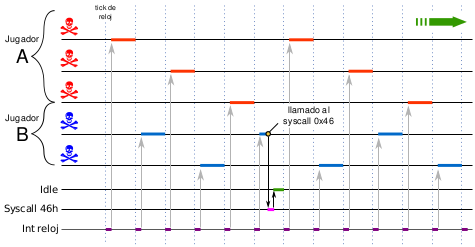
\includegraphics[width=0.7\textwidth]{images/scheduler}
  \caption{Diagrama de Tareas}
\end{figure}

Mantiene un contador para saber por cuantos ciclos de clock se ha ejecutado la tarea actual. A su vez, mantiene un flag para identificar a que jugador pertenece la ultima tarea que ha sido ejecutada. Para identificar que tarea ejecutar, itera sobre los piratas del jugador a partir del actual. Una tarea es ejecutada a lo sumo \texttt{SCHEDULER\_TASK\_TICKS} ciclos de clock. Esto esta definido en \texttt{defines.h}.

\subsection{Estructuras}

\subsection{Funciones Auxiliares}

\subsection{Tareas}

\subsubsection{Idle}

\subsubsection{Explorador}

\subsubsection{Minero}
